\section{Methods}

\begin{figure}[!h]
    \centering
    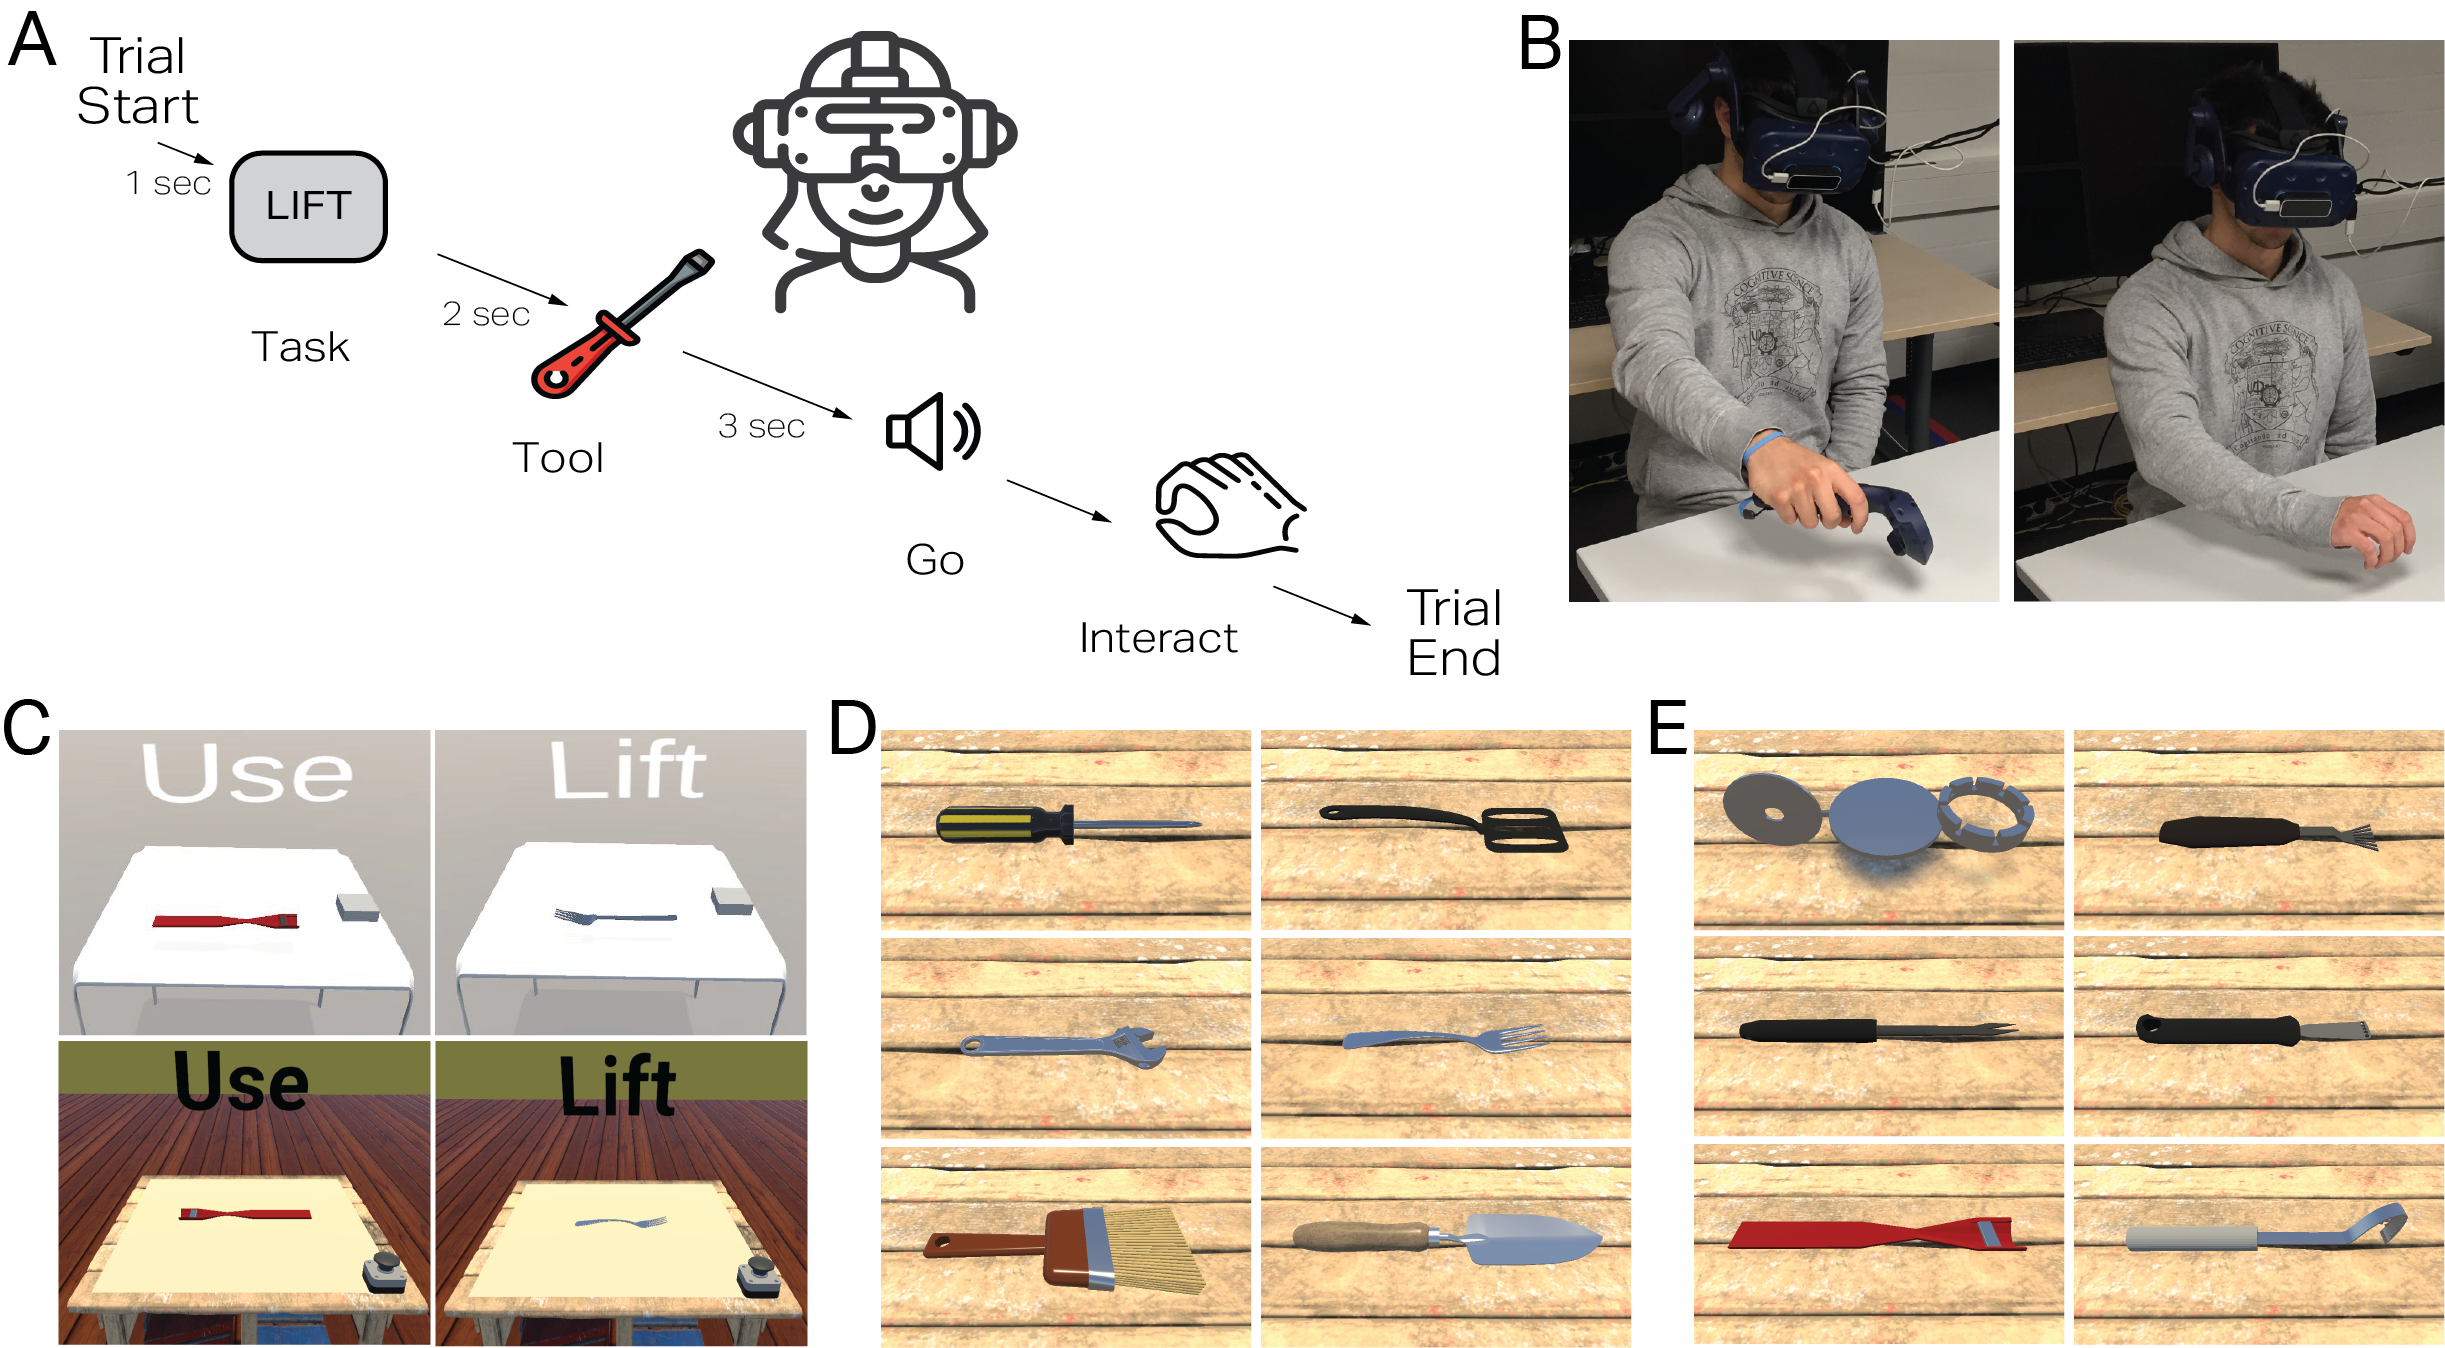
\includegraphics[width=1\linewidth]{source/figures/setup/Methods_1.png} \\
    \caption[]{Experimental Task. In two virtual environments participants interacted with tools in two ways (LIFT, USE). The tools were categorized based on familiarity (FAMILIAR, UNFAMILIAR) and presented to the participants in two orientations (HANDLE LEFT, HANDLE RIGHT). The two virtual environments differed based on the mode of interaction and perceived realism, wherein in one experiment, subjects’ hand movements were rendered virtually using the HTC-VIVE controllers. In the other experiment, the hands were rendered using LeapMotion, allowing finer hand and finger movements. \textbf{Panel A} shows the timeline of a trial. \textbf{Panel B} shows a subject in real-life performing the task in the two experiments. \textbf{Panel C} shows the differences in realism in the two experiments; TOP panels correspond to experiment with the controllers, the USE and LIFT conditions for an UNFAMILIAR and FAMILIAR tool, respectively with the tool handles presented in two different orientations. BOTTOM panels illustrate the three different conditions in a more realistic environment with LeapMotion as the interaction method. \textbf{Panel D} Familiar tools, from top-left: screwdriver, spatula, wrench, fork, paintbrush, trowel. \textbf{Panel E} Unfamiliar tools, from top-left: spoke-wrench, palette knife, daisy grubber, lemon zester, flower cutter, fish scaler.
    }
    \label{figure:task}
\end{figure}

\subsection{Experimental Task}

Subjects were seated in a virtual environment where they had to interact with the presented tool by either lifting or pretending its use.  The time course of the trials is illustrated in Figure \ref{figure:task}A. At the start of a trial, subjects saw the cued task for 2 sec after which the cue disappeared, and a tool appeared on the virtual table. Subjects were given 3 sec to view the tool, after which there was a beep (go cue) which indicated that they could start manipulating the tool based on the cued task. Subjects were seated in a virtual environment where they had to interact with the presented tool by either lifting or pretending its use. After interacting with the tool, subjects pressed a button on the table to start the next trial.  

\subsection{Participants}

For experiment-I with the HTC Vive controller’s interaction method, we recruited 18 participants ( 14 females, mean age=23.68, SD=4.05 years). For experiment-II with the interaction method of LeapMotion, we recruited 30 participants (14 female, mean age=22.7, SD=2.42 years).  All participants were recruited from the University of Osnabr{\"u}ck and the University of Applied Sciences Osnabr{\"u}ck. Participants had a normal or corrected-to-normal vision and no history of neurological or psychological impairments. All of the participants were right-handed. They either received a monetary reward of C10 or one participation credit per hour. Before each experimental session, subjects gave their informed consent in writing. They also filled out a questionnaire regarding their medical history to ascertain they did not suffer from any disorder/impairments which could affect them in the virtual environment. Once we obtained their informed consent, we briefed them on the experimental setup and task.

\subsection{Experimental Design and Procedure}

The two experiments differed based on the realism of the action affordance and the environment. Figure \ref{figure:task}B illustrates the physical setup of the participants for the two experiments. In experiment-I, subjects interacted with the tool models using the HTC Vive VR controllers. While in experiment II, subjects’ hand movements were captured by LeapMotion. 

Figure \ref{figure:task}C  illustrates two exemplar trials from the experiments. We used a 2x2x2 experimental design for both experiments, with factors task, tool familiarity, and handle orientation. Factor task had two levels: LIFT and USE. In the LIFT conditions, we instructed subjects to lift the tool to their eye level and place it back on the table. In the USE task, they had to pantomime using the tool to the best of their knowledge. Factor familiarity had two levels, FAMILIAR and UNFAMILIAR, which corresponded to tools either being everyday familiar tools or tools that are not seen in everyday contexts and are unfamiliar. The factor handle orientation corresponded to the tool handle, which was presented to the participants either on the LEFT or the RIGHT. Both experiments had 144 trials per participant, with an equal number of trials corresponding to the three factors. Subjects performed the trials over six blocks of 24 trials each. 
We measured the eye movements and hand movements simultaneously while subjects performed the experiment. We calibrated the eye-trackers at the beginning of each block and ensured that the calibration error was less than 1 degree of the visual angle. At the beginning of the experiment, subjects performed three practice trials with a hammer to familiarize themselves with the experimental setup and the interaction method. Each experiment session lasted for approximately an hour. After that, subjects filled out a questionnaire to indicate their familiarity with the 12 tools used in the experiment. They responded to the questionnaire based on a scale of 5-point Likert-like scale where 1 corresponded to “I have never used it or heard about it,” and 5 referred to “I see it every day or every week.”

\subsection{Experimental Stimuli}

The experimental setup consisted of a virtual table that mimicked the table in the real world. The table’s height, width, and length were 86cm, 80cm, and 80cm, respectively. In experiment-I, subjects were present in a bare room with grey walls and constant illumination. They sat before a light grey table, with a dark grey button on their right side to indicate the end of the trial. Similarly, in experiment-II, subjects were present in a more immersive, realistic room. They sat in front of a wooden workbench with the exact dimensions of the real-world table and a buzzer on the right to indicate the end of a trial. We displayed the task (USE or LIFT) over the desk 2m away from the participants for both experiments. 

For both experiments, we used the tool models as presented in \citet{Belardinelli2016-xb}. Six of the tools were categorized as familiar (Figure \ref{figure:task}D) and the other six as unfamiliar (Figure \ref{figure:task}E). We further created bounding box colliders that encapsulated the tools to capture the gaze position on the tool models. The mean length of the bounding box was 34.04cm (SD=5.73), mean breadth=7.60cm (SD=3.68) and mean height= 4.17cm (SD=2.13). To determine the tool effector and tool handle regions of interest, we halved the length bounding box colliders from the center of the tool and took one half as the effector and the other half as the handle. This way we refrained from making arbitrary-sized regions-of-interest for the different tool models. 

\subsection{Apparatus}
For both experiments, we used an HTC Vive head-mounted display (HMD)($110^\circ$ field of view, 90Hz, resolution 1080 x 1200 px per eye) with a built-in Tobii  eye-tracker \footnote{\href{https://enterprise.vive.com/us/product/vive-pro-eye/}{https://enterprise.vive.com/us/product/vive-pro-eye-office/}}. The HTC Vive Lighthouse tracking system provided positional and rotational tracking and was calibrated for a 4m x 4m space. For calibration of the gaze parameters, we used 5-point calibration function provided by the manufacturer. To make sure the calibration error was less than $1^\circ$, we performed a 5-point validation after each calibration. Due to the nature of the experiments, which allowed a lot of natural head movements, the eye tracker was calibrated repeatedly during the experiment after each block of 36 trials. We designed the experiment using the Unity3D game engine \footnote{\href{www.unity.com}{Unity, www.unity.com}} (v2019.2.14f1) and controlled the eye-tracking data recording using HTC VIVE Eye Tracking SDK SRanipal\footnote{\href{https://developer.vive.com/resources/vive-sense/sdk/vive-eye-tracking-sdk-sranipal/}{SRanipal, developer.vive.com/resources/vive-sense/sdk/vive-eye-tracking-sdk-sranipal/}} (v1.1.0.1)

For experiment-I, we used HTC Vive controller\footnote{\href{https://valvesoftware.github.io/steamvr_unity_plugin/articles/Quickstart.html}{SteamVR, https://valvesoftware.github.io/steamvr\_unity\_plugin/articles/Quickstart.html}} (version 2.5) to interact with the tool. The controller in the virtual environment was rendered as a gloved hand. When participants pulled the trigger button of the controller with their right index finger, their right virtual hand made a power grasp action. To interact with the tools, subjects pulled the trigger button of the controller over the virtual tools and the rendered hand grasped the tool handle.

Similarly, in experiment-II, we used LeapMotion\footnote{\href{https://developer.leapmotion.com/unity}{LeapMotion Unity modules, https://developer.leapmotion.com/unity}} (version 4.4.0)  to render the hand in the virtual environment. Here, subjects could see the finer hand and finger movements of their real-world movements rendered in the virtual environment. When participants made a grasping action with their hand over the virtual tool handle, the rendered hand grasped the tool handle in the virtual environment.

\subsection{Data pre-processing}

\subsubsection{Gaze Data}

As a first step, using eye-in-head 3D gaze direction vector for the cyclopean eye we calculated the gaze angles in degrees for the horizontal $\theta\textsubscript{h}$ and vertical $\theta\textsubscript{v}$ directions. All of the gaze data was sorted by the timestamps of the collected gaze samples. The 3D gaze normals are represented as $(x, y, z)$ a unit vector that defines the direction of the gaze in VR world coordinates. In our setup, the x coordinate corresponds to the left-right direction, y in the up-down direction, z in the forward-backward direction. The formulas used for computing the gaze angles are as follows:

 \begin{equation*}\label{eq:h_angle}
     \theta\textsubscript{h} = \frac{180}{\pi} \arctan{\frac{x}{z}}
 \end{equation*}   
  \begin{equation*}\label{eq:v_angle}
     \theta\textsubscript{v} = \frac{180}{\pi} \arctan{\frac{y}{z}} 
 \end{equation*}   
 
Next, we calculated the angular velocity of the eye in both the horizontal and vertical coordinates by taking a first difference of the angular velocity and dividing by the difference between the timestamp of the samples using the formula below:
\begin{equation*}\label{eq:h_vel_angle}
    \omega\textsubscript{h} = \Delta\theta\textsubscript{h} / \Delta t
 \end{equation*}  
 \begin{equation*}\label{eq:v_vel_angle}
     \omega\textsubscript{v} = \Delta\theta\textsubscript{v} / \Delta t
 \end{equation*}  

Finally, we calculated the magnitude of the angular velocity ($\omega$) at every timestamp from the horizontal and vertical components using:
\begin{equation*}\label{eq:vel_angle}
     \omega = \sqrt{\omega_h^2 + \omega_v^2}
 \end{equation*}  

To classify the fixation and saccade-based samples, we used an adaptive threshold method for saccade detection described by \citet{Voloh2020-nz}.  We selected an initial saccade velocity threshold $\theta\textsubscript{0}$ of 200 $\circ$/sec. All eye movement samples with an angular velocity of less than $\theta\textsubscript{0}$ were used to compute a new threshold $\theta\textsubscript{1}$. $\theta\textsubscript{1}$ was three times the median absolute deviation of the selected samples. If the difference between $\theta\textsubscript{1}$ and $\theta\textsubscript{0}$ was less than 1 $\circ$/sec $\theta\textsubscript{1}$ was selected as the saccade threshold else, $\theta\textsubscript{1}$ was used as the new saccade threshold and the above process was repeated. This was done until the difference between $\theta\textsubscript{n}$ and $\theta\textsubscript{n+1}$ was less than or equal to 1 $\circ$/sec. This way we arrived at the cluster of samples that belonged to fixations and the rest were classified as saccades.

After this, we calculated the duration of the fixations and removed those fixations that had a duration less than 50 ms or were larger than 3.5 times the median absolute deviation of the fixation duration. For further data analysis, we only considered those fixations that were positioned on the 3D tool models. We further categorized the fixations based on their position on the tool, i.e., whether they were located on the effector or handle of the tool.


\subsection{Data Analysis}\label{sec:data_analysis}

\subsubsection{Odds of Fixations in favor of tool effector}

After cleaning the dataset, we were left with 2174 trials from 18 subjects in experiment-I and 3633 trials from 30 subjects in experiment-II. For both experiments, we analysed the fixations in the 3 second period from the tool presentation till the go cue. For the two experiments, we modeled the linear relationship of the log of odds of fixations on the effector of the tools and the task cue (LIFT, USE), the familiarity of the tool (FAMILIAR, UNFAMILIAR), and orientation of the handle (LEFT, RIGHT). All within-subject effects were also modeled with random intercepts and slopes based on the subjects. We were also interested in modeling the random effects based on the tool to assess the differential effects on the individual tools. We did not have enough data to estimate random item effects, so we fitted a random intercept for the 12 tools.

We used effect coding \citep{Schad2018-av} to construct the design matrix for the linear model, where we coded the categorical variables LIFT, FAMILIAR, RIGHT to -0.5 and USE, UNFAMILIAR, LEFT to 0.5. This way, we could directly interpret the regression coefficients as main effects. The model fit was performed using restricted maximum likelihood (REML) estimation \citep{Corbeil1976-qq} using the lme4 package (v1.1-26) in R 3.6.1. We used the L-BFGS-B optimizer to find the best fit using 10000 iterations. Using the Satterthwaite method \citep{Luke2017-pz}, we approximated degrees of freedom of the fixed effects. For both experiments, the Wilkinson notation \citep{Wilkinson1973-ex} of the model was:

\begin{gather*}\label{eq:data_model}
    log \frac{p(fixations \quad on \quad effector)}{p(fixations \quad on \quad handle)} \sim 1 + task * familiarity * handle\_orientation \\ + (1 + task * familiarity * handle\_orientation | Subject) \\ + (1 | tool)
 \end{gather*}

As we used effects coding, we can directly compare the regression coefficients of the two models. The fixed-effect regression coefficients of the two models would describe the differences in log-odds of fixations in favor of tool effector for the categorical variables task, familiarity, and handle orientation.


\subsubsection{ Spatial bias of fixations on the tools}

In this analysis, we wanted to assess the effects of task, tool familiarity, and handle orientation on the eccentricity of fixations on the tools. To do this, we studied the fixations from the time when the tool was visible on the table (3s from the start of trial) till the go cue indicated when subjects could start manipulating the tool. We divided this 3s period into 20 equal bins of 150ms each. For each trial and time bin, we calculated the median distance of the fixations from the tool center. Next, we normalized the distance with the length of the tool so that we could compare the fixation eccentricity across different tools.

To find the time-points where there were significant differences for the 3 conditions and their interactions, we used the cluster permutation method. Here, we use the t-statistic as a test statistic for each time-bin, where t is defined as:


\begin{gather*}\label{eq:cluster_permutation}
 t = \sqrt{N} * \frac{x}{\sigma}
 \end{gather*}

and, x is the mean difference between conditions, and $\sigma$ is the standard deviation of the mean and N is the number of subjects. We used a threshold for t at 2.14 which corresponds to the t-value at which the p-value is 0.05 in the t-distribution. We first found the time-bins where the t-value was greater than the threshold. Then, we computed the sum of the t-values for these clustered time-bins which gave a single value that represented the mass of the cluster. Next, to assess the significance of the cluster, we permuted all the time-bins across trials and subjects and computed the t-values and cluster mass for 1000 different permutations. This gave us the null distribution over which we compared the cluster mass shown by the real data. We considered the significant clusters to have a p-value less than 0.05. In the results, we report the range of the significant time-bins for the 3 different conditions and their interactions and the corresponding p-values. 
